\documentclass[14pt]{beamer}
\title{Maze}
\date{30-03-2021}
\author[Bvrith]{Harini: 19WH1A0510: CSE \\ Mounika: 20WH5A0513: CSE \\ Sai Preethi: 19WH1A0215: EEE  \\ Sanjana: 19WH1A1263: IT \\  Nidhi: 19WH1A0507: CSE }
\usepackage{xcolor}
\definecolor{blendedblue}{rgb}{0.2,0.2,0.7}
\institute{\normalsize{\color{blendedblue}{BVRIT HYDERABAD College of Engineering for Women}}}
\usefonttheme{serif}
\usepackage{bookman}
\usepackage{hyperref}
\usepackage[T1]{fontenc}
\usepackage{graphicx}
\usecolortheme{orchid}
\beamertemplateballitem
\graphicspath{./home/user/Desktop/maze}
\graphicspath{./home/user/Desktop/maze}
\graphicspath{./home/user/Desktop/maze}
\graphicspath{./home/user/Desktop/maze}
\graphicspath{./home/user/Desktop/maze}
\graphicspath{./home/user/Desktop/maze}
\graphicspath{./home/user/Desktop/maze}

\begin{document}
    \begin{frame}
        \titlepage
    \end{frame}
    \begin{frame}
	\frametitle{Problem Statement}
        \begin{itemize}
	    \item A person placed at (0, 0) in a square matrix of order N*N, has to reach the destination at (n-1, n-1)
	    \item Find a possible path that the person can take to reach from source to destination
	    \item Directions in which the person can move are ‘U'(up), ‘D'(down), ‘L’ (left), ‘R’ (right)
	\end{itemize}
    \end{frame}
    \begin{frame}
	    \frametitle{Problem Statement}
	    \begin{figure}[htp]
                        \centering
                         \includegraphics[width=10cm]{maze1.png}
			 \caption{Maze Example}
                 \end{figure}
    \end{frame}
    \begin{frame}
	\frametitle{Approach}
	\begin{itemize}
		\item Start from the source 
		\item Move in a direction where the path is not blocked (not 0)
		\item Reach the destination to win the game
	\end{itemize}
    \end{frame}
    \begin{frame}
	\frametitle{Statistics}
	\begin{itemize}
		\item Lines of Code - 163
		\item Number of functions - 10
	\end{itemize}
    \end{frame}
    \begin{frame}
	\frametitle{Tools}
	\begin{itemize}
		\item OS - Windows 10
		\item Programming language (Python Version 3.8.1)
		\item Libraries - numpy, pygame
		\item Modules - random, mixer, sys
	\end{itemize}
    \end{frame}
    \begin{frame}
        \frametitle{Learnings}
	\begin{itemize}
	    \item Backtracking 
	    \item Generating random matrices
	    \item Embedding Audio 
	    \item Usage of pygame
	    \item Working on GIT, Latex
	\end{itemize}
    \end{frame}
    \begin{frame}
	\frametitle{Challenges}
        \begin{itemize}
	    \item Implementing Recursion
	    \item Icon movement 
	    \item Path color generation 
	    \item Exiting game window 
		\item GIT - pushing files to gitlab
        \end{itemize}
    \end{frame}
    \begin{frame}
	\frametitle{GIT Repo}
	    \url{https://gitlab.com/19wh1a0507/maze}
	\begin{figure}[htp]
                        \centering
                         \includegraphics[width=10cm]{repo.jpeg}
                 \end{figure}
    \end{frame}
    \begin{frame}
	\frametitle{Demo}
	     \begin{figure}[htp]
                        \centering
                         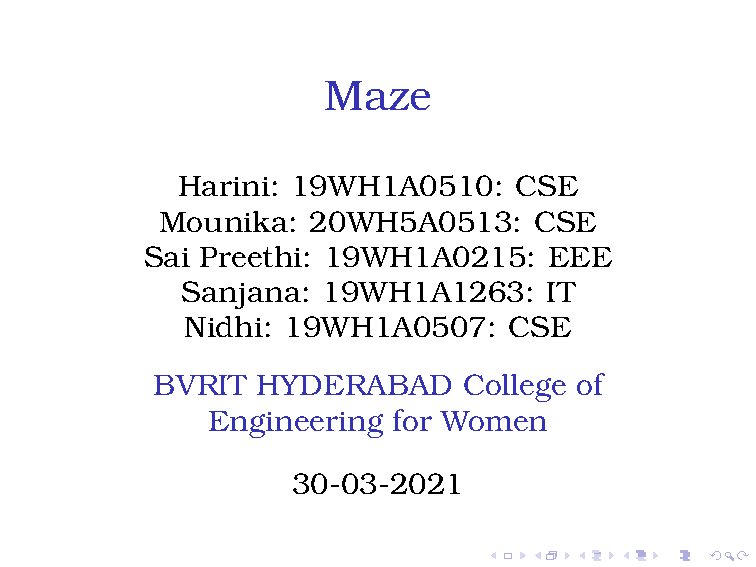
\includegraphics[width=8cm]{maze.png}
                 \end{figure}	
    \end{frame}
    \begin{frame}
	\frametitle{Demo}
	     \begin{figure}[htp]
                        \centering
                         \includegraphics[width=8cm]{maze_.png}
                 \end{figure}	
    \end{frame}
    \begin{frame}
	\begin{center}
	     THANK YOU
	\end{center}
    \end{frame}
\end{document}

